% Build: latexmk -pdf -interaction=nonstopmode -halt-on-error accord.tex
% Self-contained article: embedded bibliography and vector diagram.
\documentclass[11pt,letterpaper]{article}
\usepackage[T1]{fontenc}
\usepackage[utf8]{inputenc}
\usepackage{lmodern,microtype}
\usepackage[margin=1in,headheight=15pt]{geometry}
\usepackage{amsmath,amssymb,amsthm,mathtools}
\usepackage{booktabs,tabularx,longtable,array,enumitem}
\usepackage{xcolor,listings,tikz,needspace,fancyhdr,titlesec,etoolbox}
\usetikzlibrary{arrows.meta,positioning}
\usepackage{xurl}
\usepackage[colorlinks=true,linkcolor=blue!40!black,citecolor=blue!40!black,urlcolor=blue!40!black]{hyperref}
\usepackage{bookmark}
\definecolor{ink}{HTML}{173448}
\definecolor{accent}{HTML}{227A80}
\definecolor{pale}{HTML}{F1F5F6}
\definecolor{muted}{HTML}{52646F}
\titleformat{\section}{\Large\sffamily\bfseries\color{ink}}{\thesection}{.6em}{}
\titleformat{\subsection}{\large\sffamily\bfseries\color{ink}}{\thesubsection}{.6em}{}
\titleformat{\subsubsection}{\normalsize\sffamily\bfseries}{\thesubsubsection}{.6em}{}
\pretocmd{\section}{\Needspace{10\baselineskip}}{}{}
\pretocmd{\subsection}{\Needspace{4\baselineskip}}{}{}
\setlength{\parindent}{0pt}
\setlength{\parskip}{.38em}
\setlength{\emergencystretch}{2em}
\setcounter{tocdepth}{1}
\setlist{nosep,leftmargin=1.5em}
\renewcommand{\arraystretch}{1.15}
\newcolumntype{Y}{>{\raggedright\arraybackslash}X}
\newcolumntype{P}[1]{>{\raggedright\arraybackslash}p{#1}}
\newcommand{\code}[1]{\nolinkurl{#1}}
\newcommand{\Accord}{\textsc{Accord}}
\newcommand{\N}{\mathbb N}
\newcommand{\Z}{\mathbb Z}
\newcommand{\Q}{\mathbb Q}
\newcommand{\R}{\mathbb R}
\newcommand{\C}{\mathbb C}
\newcommand{\sem}[1]{[\![#1]\!]}
\newcommand{\coeff}[2]{[#1^{#2}]}
\newcommand{\invfact}[1]{\iota\!\left(\frac{1}{#1!}\right)}
\newcommand{\decision}[1]{\par\smallskip\textbf{Design decision.} #1\par\smallskip}
\newtheorem{proposition}{Proposition}[section]
\newtheorem{lemma}[proposition]{Lemma}
\newtheorem{theorem}[proposition]{Theorem}
\theoremstyle{definition}
\newtheorem{definition}[proposition]{Definition}
\newtheorem{example}[proposition]{Example}
\lstset{basicstyle=\small\ttfamily,columns=fullflexible,keepspaces=true,
 breaklines=true,showstringspaces=false,frame=single,
 rulecolor=\color{accent!35},backgroundcolor=\color{pale},
 aboveskip=.7em,belowskip=.7em,framesep=6pt,xleftmargin=6pt,xrightmargin=6pt}
\BeforeBeginEnvironment{lstlisting}{\par\noindent\begin{minipage}{\linewidth}}
\AfterEndEnvironment{lstlisting}{\end{minipage}\par}
\pagestyle{fancy}
\fancyhf{}
\fancyhead[L]{\small\sffamily Accord: mathematics with certified computation}
\fancyhead[R]{\small\sffamily Round-two proposal}
\fancyfoot[C]{\thepage}
\hypersetup{pdftitle={Accord: A Mathematical Language of Certified Transformations},pdfauthor={ChatGPT, prepared for Vladimir Reshetnikov},pdfsubject={Second-round proof-language proposal; Lean, Leant, verified computer algebra}}

\begin{document}
\begin{titlepage}
\color{ink}
{\sffamily\large PROOF-LANGUAGE DESIGN \quad / \quad SECOND ITERATION\par}
\vspace{1.05in}
{\sffamily\bfseries\fontsize{37}{42}\selectfont Accord\par}
\vspace{.20in}
{\sffamily\bfseries\fontsize{25}{30}\selectfont A Mathematical Language\\of Certified Transformations\par}
\vspace{.32in}
{\sffamily\Large A proof assistant and computer algebra workbench\\with explicit meaning, guards, and guarantees\par}
\vspace{.55in}
{\large A proposal grounded in ProveIt, Leant,\\and both Brainstorm synthesis reports\par}
\vfill
\rule{\textwidth}{.8pt}
\vspace{.15in}
Prepared for Vladimir Reshetnikov\par
5 September 2026, Pacific time\par
\vspace{.2in}
{\small\color{muted}
Status: design specification and source-based analysis, with mathematical
worked examples and an executed exact-arithmetic companion. The proposed
language, Lean adapters, and certified CAS are not implemented here.
The companion's 267 checks are Python checks, not kernel-checked proofs.
}
\end{titlepage}

\begingroup\small\setlength{\parskip}{.25em}
\begin{abstract}
A more natural proof language should not merely hide Lean tactics. It should let
mathematicians name objects, choose representations, calculate, and organize
arguments while preserving exactly what each operation establishes. The first
Brainstorm round has already identified a strong common core: fixed statements,
scoped obligations, theorem-backed methods, retained evidence, and fair comparison
with equally equipped Lean. This article accepts that core and proposes a more
specific second-round direction: a \emph{relational proof-and-computation language}.

In \Accord, every computational result states its semantic relation to the input:
equality, equivalence of solution sets, a witnessed property, a certified enclosure,
or agreement through a specified formal order. Guards, locality, precision, and
solution completeness are part of the interface rather than informal annotations.
Mathematical objects retain stable semantic definitions while exposing certified
representations suited to computation. Ordinary theorem applications, verified
algorithms, external certificate-producing engines, and Leant synthesis share one
acceptance boundary but retain different evidence and completeness claims.

Worked examples cover parameter-degenerate equations, radical branches, binomial
inversion, Abel-series coefficients over arbitrary commutative rational algebras,
local autonomous differentiation, Lambert derivative polynomials, and certified
root enclosures. The proposal gives concrete policies for representation coherence,
definition authoring, exact suggestion replay, proof-document coverage, dependency
upgrades, and all twenty-two questions posed by the two syntheses. A staged
implementation and an ablation-based evaluation could establish whether the
result deserves a new authored surface or should remain a Lean library and
mathematical document view.
\end{abstract}

\section*{The proposal in one page}
\addcontentsline{toc}{section}{The proposal in one page}
\textbf{Thesis.} Make the unit of interaction a \emph{mathematical transformation
with a declared guarantee}, not a tactic invocation and not an unqualified CAS
answer. The source should expose choices that can change the mathematics; the
system should reconstruct and retain their formal consequences.

The characteristic interaction is not simply ``prove this.'' It is: ``work with
this formal series through degree nine,'' ``solve this equation for all parameter
cases,'' ``differentiate this identity near this point,'' or ``compute an enclosure
of the already specified root.'' Each request selects a precise relation and a
scope. The checker never upgrades a weaker result to the stronger relation the
reader might have inferred.

\textbf{Five concrete additions to the first-round core.}
First, a result vocabulary distinguishes exactness from completeness: finding an
exact root does not enumerate all roots. Second, a definition package binds a
semantic object to proved observation and representation interfaces, so repeated
casts and normalization choices need not be authored at every use. Third, a
precision-and-locality discipline prevents a finite jet, pointwise identity, or
numerical sample from masquerading as a stronger theorem. Fourth, CAS integration
accepts either proved algorithms with justified executions or independent
certificates; neither native execution nor a solver's completeness flag becomes
an undisclosed axiom. Fifth, the proposal chooses specific defaults for the
syntheses' open questions, with experiments that could overturn those choices.

\textbf{First implementation.} Build a Lean package with a small claim/operation
record, one local-calculus wrapper, one guarded algebra certificate path, and one
formal-series observation interface. Give these to ordinary Lean and to the new
surface. Connect Leant through exact scoped obligations, not through authoritative
pretty-printed goals. A finished example must survive replay with discovery
services disabled and must reject its nearby invalid variants.

\textbf{Stopping rule.} New syntax is not a success condition. If shared libraries,
certified computation, and a rendered mathematical view give the benefit without
improving authoring through a new surface, ship those components instead.

\endgroup
\clearpage
\begingroup
\small\setlength{\parskip}{0pt}
\tableofcontents
\endgroup
\clearpage

\section{What was read, and what the evidence supports}\label{sec:evidence}
\subsection{The source boundary}
Both requested synthesis reports were read closely, including their revisions,
Leant discussions, caveats, and questions for the next iteration. The retrieved
Brainstorm revision was \code{494be9d5ab41a5ae219fc6f800e6aee3c93bce39}.
The two documents are \emph{Mathematical Ideas, Checked Evidence} and
\emph{Nine Blueprints for a Mathematician's Proof Language over Lean}
\cite{synthesis,review}. Individual proposals are discussed only through those
syntheses; this article does not claim a fresh full reading of all nine originals.

The direct ProveIt inspection used revision
\code{24ce8bd743eaab64a91ce90725ea00f498d319d2}, as returned by its main-branch
endpoint. Three complete modules supplied contrasting examples:
\code{BinomialInversion.lean}, \code{AbelPolynomialSeries.lean}, and
\code{AutonomousIteratedDeriv.lean}\cite{pbinomial,pabel,pode}.
The syntheses also discuss a newer local ProveIt checkout, \code{7c4e3f10}; their
local audit and this article's fetched source are not silently treated as the same
snapshot.

Leant inspection used revision
\code{3a40904be8a410d832d9ab6900b3d3e7b425eccb}, specifically the verification
scheduler, the engine's interface and provenance records, and the tactic-suggestion
path in \code{Main.hs}\cite{lverification,lengine,lmain}. The syntheses describe
additional modified and untracked working-tree code, including behavioral-query
work. Those descriptions remain attributed to the reports; they are not evidence
that the feature is present in the pinned committed files inspected here.

This is a static source review. No ProveIt or Leant build was run, and no proposed
Accord block was elaborated by Lean. The separate arithmetic companion was run;
its deliberately narrower scope is specified in Section~\ref{sec:exhibits}.

\subsection{What survives the first round}
The first synthesis formulates six shared commitments more cautiously than a vote
for nine competing languages: use Lean, expose mathematical assertions, retain
scoped obligations, fix meaning at the search boundary, preserve accepted evidence,
and evaluate against a shared-library Lean baseline. The second supplies a finer
feature matrix, an audit of source patterns, an annotated-theorem implementation
idea, and a stronger emphasis on definitions\cite{synthesis,review}.

These are a productive starting point, not findings that require a tenth manifesto
to rediscover. In particular, the repeated relative-soundness argument is necessary
but not a large research contribution: correctly applying checked terms to a
checked dependent telescope yields a checked result. The engineering questions
are whether the telescope matches the author's meaning, whether computation
preserves that meaning, and whether the visible argument describes what was
actually accepted.

The reported lexical audit classified 90,637 tactic-like entries in 1,004
FabiusFunction files; 32.3\% fell into families selected as possible reconstruction
targets. Both reports ultimately caution that this is not measured removable
work\cite{synthesis,review}. I use the audit to motivate examples, not to predict a
one-third reduction in effort. Similarly, shared design language across reports
is not independent empirical validation of usability.

\subsection{Three source observations that constrain the design}
\textbf{Some apparent verbosity protects generality.}
Binomial inversion is available for sequences in an arbitrary additive commutative
group, with integer scalar actions. Its cast version works in an arbitrary
commutative ring. A CAS interface that translates everything to a rational field
would change the mathematical theorem, even if its output looked shorter
\cite{pbinomial}.

\textbf{The chosen solution is not always the theorem's subject.}
The Abel module constructs a canonical formal series but proves its coefficient
formula for \emph{any} series satisfying the functional equation. Its coefficient
ring is any commutative \(\Q\)-algebra, not necessarily a field. The long-looking
algebra-map and factorial steps enforce exactly that generality\cite{pabel}.

\textbf{Locality is mathematics, not clutter.}
The autonomous-derivative theorem needs equality near the differentiation point
and derivatives of auxiliary functions only at values reached by the solution.
Its short proof explicitly constructs an eventual equality and then applies the
chain rule\cite{pode}. The appropriate improvement is an interface that preserves
this locality, not a rewrite that silently assumes global differentiability.

\section{The design delta: from proof steps to mathematical transformations}\label{sec:delta}
\subsection{Why a proof assistant--CAS hybrid is the right question}
A proof assistant normally asks whether a specified statement has evidence. A CAS
interaction often asks for a new expression, object, decomposition, solution, or
approximation. A mathematician moves between these activities continuously. One
computes a few coefficients, recognizes a pattern, selects an invariant, proves
a recurrence, and then uses the proved recurrence for larger computations.

The relevant distinction is therefore not ``reasoning versus calculation.'' It is
\emph{which guarantee was requested, which guarantee was established, and which
choices have become part of the argument}. An exact rational number, a formal
power series, a real root, and a finite precision approximation can coexist in one
notebook without having interchangeable semantics.

\Accord\ is a working name for that interface. Its central object is a
\emph{transformation record} linking a fixed input to an output under a specified
relation, with all required premises. It can support proof-only use, computation-only
exploration, and a combined published proof document.

\subsection{What is inherited and what is proposed here}
\begin{tabularx}{\textwidth}{@{}P{.28\textwidth}Y@{}}
\toprule
Inherited from the syntheses & Specific second-round refinement \\
\midrule
Statement seals & Seal the semantic object and requested relation, including
solution completeness, locality, and precision.\\
Theorem-backed methods & Use three backends under one interface: theorem
application, proved algorithm, and certificate checker. Their evidence differs.\\
Certified views & Anchor each view to specified observations of a stable object;
compose only with proved relation transport and discharged guards.\\
Proof/data distinction & Distinguish witness discovery, construction, canonical
selection, and all-solution computation in the authored operations.\\
Scoped obligations & Make conditional computational results usable as implications,
without installing their unresolved guards as assumptions.\\
Evidence replay & Retain a relation-specific certificate and checker identity as
well as the resulting Lean evidence; keep discovery-independent replay distinct
from computation-free replay.\\
Definition experiment & Start with observation templates, especially coefficients,
finite indexing, and local function specifications, rather than a new general
language for every definition.\\
\bottomrule
\end{tabularx}

These are integration and interface proposals, not claims to have invented
reflection, structured proofs, refinement relations, or proof-carrying computation.
The contribution to this campaign is to make their consequences precise enough
to build and falsify.

\subsection{The computational guarantee is two-dimensional}
Consider four outputs for \(x^2=2\). A decimal approximation suggests where a root
lies. An exact algebraic number with a proof of its square supplies one root. A
positive-root contract chooses a branch. A complete solution-set theorem identifies
both roots and proves that there are no others. Calling all four ``verified''
would hide their principal difference.

Accordingly, an accepted result records a \emph{semantic guarantee} and an
\emph{evidence mechanism}. Exactness, completeness, uniqueness, and error width
belong to the former. A kernel-checked theorem, a reflective checker, or a
compiler-trusting execution profile belongs to the latter. A method may be fully
verified for a deliberately incomplete specification. That does not make its
answer complete for a stronger request.

\decision{Do not expose a single undifferentiated \code{compute} success flag.
Let the requested relation determine the output type and the required evidence.}

\section{The language a mathematician would see}\label{sec:surface}
\subsection{A small stored language, with richer mathematical rendering}
The first frontend should reuse Lean expressions and types. A small proof-block
syntax supplies claims, constructions, scoped transformations, and calculations.
The printed document can render these as familiar mathematical sentences, while
the editor exposes the exact expression and its interpretation on demand. Prose
written outside the controlled grammar is commentary, not automatically certified
mathematics.

The following is proposed syntax, not executable Lean:
\begin{lstlisting}
context (a b : Real)

solve x : Real where a*x = b completely as S
  split on a = 0
  case a != 0:
    return singleton (b/a) by field_equivalence
  case a = 0:
    split on b = 0
    case b = 0:  return all
    case b != 0: return empty

claim characterization:
  forall x, a*x = b iff x in S
  from S.certificate
\end{lstlisting}

Here \code{completely} is not praise for the solver. It requires an equivalence
between the original predicate and membership in the returned set. Replacing the
output with a single root changes the task and must be rejected unless the author
changes the source.

A proof that needs only one witness can say so:
\begin{lstlisting}
obtain r with 1 < r and r < 3/2 and r^3-r-1 = 0
  by intermediate_value

approximate r within 1/2^20 as I
  by rational_bisection
\end{lstlisting}
The first operation introduces a witness from existential evidence, scoped to the
proof. The second computes an enclosure of that already specified witness; it does
not replace \(r\) with a rational approximation.

\subsection{A deliberate vocabulary for mathematical choices}
\code{Claim} introduces a proposition whose evidence is required even if unused.
\code{Obtain} eliminates an existential into an allowed proof scope.
\code{Construct} produces a data object together with its specification, such as a
finite map, a polynomial, or a computable witness. \code{Define} introduces an
accepted mathematical object and fixes its interface. These operations should not
all be hidden behind a single overloaded ``choose.'' Noncomputable choice is a
separate, disclosed construction mode.

\code{Transform} changes a representation under an explicit relation.
\code{Calculate} chains relations through registered transitivity theorems.
\code{Solve completely} requests a solution-set equivalence.
\code{Approximate} requests containment and an error or width bound.
\code{Work locally} selects a neighborhood, filter, or domain of validity.
\code{Induct} exposes the induction variable and invariant. A larger induction
motive is an editable proof-plan change, not silent routine synthesis.

These words need not all become new parser keywords. Most can initially be
attributes, commands, or code actions over ordinary Lean declarations. Their
semantic distinctions are more important than their spelling.

\subsection{Two kinds of omitted explanation}
An open claim may be discharged by any permitted proof:
\begin{lstlisting}
claim h : P by search using [h1, h2]
\end{lstlisting}
A named mathematical operation imposes a stronger construction contract:
\begin{lstlisting}
transform sum S f to sum T g
  by reindex with map phi
\end{lstlisting}
If \(\phi\) misses an endpoint, a different proof of equality does not validate the
advertised reindexing. The system should display the missing coverage premise and
offer an alternative as a changed source step. Conversely, a proof-only claim
should not be rejected merely because a different sound proof was found.

Method conformance establishes that a particular proof constructor and its
premises were used. It does not establish psychological fidelity to a human's
thought process, nor that every named premise was logically indispensable.
This limitation follows the careful distinction already made by the syntheses
\cite{synthesis,review}.

\subsection{The ordinary Lean frontend is not a second-class citizen}
The same semantic record should be attachable to an ordinary Lean \code{have},
\code{calc}, or theorem application. Existing proofs can be lifted by recognizing
assertion boundaries and registered patterns. Unrecognized tactic blocks remain
opaque leaves with exact input and output interfaces; the system must not invent
a mathematical explanation from a proof term it does not understand.

A controlled frontend and an annotated-Lean frontend can therefore share a reader
view without promising arbitrary round-trip decompilation. The subset with a
faithful editable round trip is explicitly specified. This is both a migration
strategy and the experiment that can determine whether anyone needs to type the
new surface at all.

\section{A precise core: relation-indexed tasks}\label{sec:core}
\subsection{The logical contract}
Fix a Lean environment \(E\) and an ordered local telescope \(\Gamma\). A simple
computational task has input \(x:A\), output type \(B\), and requested relation
\(R:A\to B\to\mathrm{Prop}\). An accepted result is an output \(y:B\) and a checked
term
\[
 E;\Gamma\vdash p:R(x,y).
\]
Dependent outputs use \(B(x)\) and the corresponding dependent relation. The
operational record also carries source identity, method policy, allowed
dependencies, resources, and environment identity; those fields do not replace
the logical proposition.

\begin{tabularx}{\textwidth}{@{}P{.23\textwidth}YP{.23\textwidth}@{}}
\toprule
Request & Required relation & What is not implied \\
\midrule
Normalize expression & \(\sem{e}=\sem{e'}\) in the declared domain & Validity after
guard-breaking specialization.\\
Find a witness & \(P(y)\) & Uniqueness or enumeration of all witnesses.\\
Solve completely & \(\forall z,\ P(z)\leftrightarrow z\in S\) & A preferred ordering
or canonical element of \(S\).\\
Enclose a value & \(l\le v\le u\), with a width contract & Equality of \(v\) to the
midpoint.\\
Compute a formal jet & \(f\equiv g\pmod{X^N}\) & Equality of full series or analytic
convergence.\\
Differentiate locally & A derivative or derivative identity on the stated locality &
A global identity or a selected antiderivative constant.\\
\bottomrule
\end{tabularx}

\subsection{Conditional results are useful without being promoted to facts}
A routine may return \(y\) with evidence \(G\to R(x,y)\). That is a legitimate
\emph{conditional result}. It is not a proof of \(R(x,y)\) until \(G\) is established.
The condition can be discharged from the current context, exposed as an open
obligation, or placed inside an explicit case. It cannot be added to the theorem's
hypotheses by the computation service.

For a denominator-clearing operation, the result can be stored and inspected while
\(a\ne0\) remains open. Downstream steps may reason conditionally under that guard,
but the published unconditional theorem still owes the appropriate implication
application or case coverage. Pending results do not enter the unconditional fact
index.

This approach permits useful speculative calculation without the familiar CAS
ambiguity of an answer that is merely ``generically true.'' The output can be
correct as a conditional theorem even when its guard is false in a later branch.

\subsection{Composition requires the actual relation theorem}
Suppose a first operation establishes \(R(x,y)\), a second establishes \(S(y,z)\),
and a registered theorem gives
\[
 c:\forall x\,y\,z,\ R(x,y)\to S(y,z)\to T(x,z).
\]
The composite result is \(c\,x\,y\,z\,p\,q\). The relation \(T\) is not guessed
from the word ``transform.'' Equalities, implications, inclusions, approximation
bounds, and congruences have different composition rules.

For example, from \(|x-y|\le\varepsilon\) and \(|y-z|\le\delta\), the advertised
relation must allow the accumulated bound \(\varepsilon+\delta\). From
\(P\Rightarrow Q\) and \(Q\Rightarrow R\), one obtains an implication, not an
equivalence. From two finite-precision computations, the output precision is
computed by a theorem about the operations, not copied from the more accurate
input.

\subsection{Three implementation forms, one checked result}
An ordinary method theorem already has the right shape. For example,
\(H_1\to\cdots\to H_k\to R(x,y)\) supplies both premises and proof assembly.
Binder roles identify mathematical inputs and obligations, but the theorem type
remains the authoritative logical contract.

A verified algorithm instead provides a function \(f\) and a theorem
\[
 \forall x,\ \operatorname{Pre}(x)\to R(x,f(x)).
\]
An independent certificate checker provides a decidable check and a soundness
result
\[
 \forall x\,y\,c,\ \operatorname{check}(x,y,c)=\mathrm{true}
 \to R(x,y).
\]
Both can be instantiated at the current input. When the algorithm returns guards,
branches, or richer structures, its result specification explicitly contains them.
Termination, completeness, and output-format invariants are separate theorems
when they are claimed.

\decision{Keep ordinary methods ordinary theorems. Introduce a richer computational
interface only where there is an actual algorithm, certificate format, dependent
output, or precision transformation to describe.}

\subsection{Scope and final assembly}
All obligations are closed over their authorized telescope before external
exchange. A witness for \(\forall x\,\exists y\,P(x,y)\) may depend on \(x\);
a witness for \(\exists y\,\forall x\,P(x,y)\) may not. Type dependencies are part
of the telescope, including local structures and instances that affect expressions.

A completed document is assembled by checked theorem applications and recursors,
then rechecked at its fixed target. This is the familiar conditional-assembly
argument in the first round\cite{synthesis,review}. It proves neither successful
search nor statement fidelity. The latter is addressed through semantic
interfaces, resolved displays, and explicit change review rather than by repeating
the substitution lemma at greater length.

\section{Definitions, representations, and predictable views}\label{sec:views}
\subsection{A definition package has a semantic anchor}
The definition question in both syntheses deserves an operational answer. Start
with a small package consisting of an ordinary Lean definition, named observations,
proved interface lemmas, computational representations, and a lexical display
policy. The semantic definition is the anchor. A faster representation is justified
relative to that anchor rather than becoming a replacement meaning chosen by a
solver.

For a formal series \(F\), the primary observations are its coefficients. A finite
array can represent its first \(N\) coefficients, with the contract
\[
 \operatorname{JetRep}(F,N,v)\quad\Longleftrightarrow\quad
 \forall n<N,\ v_n=\coeff Xn F.
\]
The index bound is part of the relation. It is not permissible to extend the array
with zeros and conclude that all later coefficients of \(F\) vanish.

For a finite sum, the package can adopt inclusive mathematical intervals while
providing proved bridges to the half-open ranges used by a computational routine.
For a bounded function, it can expose point evaluation and a range theorem while
keeping the chosen subtype representation behind its interface. These templates
address recurring obligations without attempting to solve definition authoring
in all of dependent type theory at once.

\begin{lstlisting}
object F : FormalSeries A
  observation coefficient n : A
  representation dense_jet N
    guarantees forall n < N, entry n = coefficient n

use representation dense_jet 10 for this calculation
retain semantic object F
\end{lstlisting}

The example is an interface declaration, not a way to conjure an arbitrary series
without a definition. The object must be a parameter, an explicit construction,
or a selected witness whose existence has already been established.

\subsection{Definitions by specification must earn existence}
The phrase ``let \(T\) be the series satisfying \(T=X\exp(-aT)\)'' can have several
formal meanings. It can introduce an arbitrary \(T\) with that hypothesis. It can
choose a witness from an existence theorem. It can define a canonical series by a
recurrence and prove the equation. Or it can use existence and uniqueness to define
an object noncomputably. These interfaces should remain distinct.

In particular, a definition command must not register its specification as an
axiom and promise to prove it later. During exploration, such an object is marked
provisional and its dependencies cannot be exported as completed results. A proved
\(\exists!T,\ P(T)\) does not by itself prescribe a computational implementation:
extracting data through classical choice and constructing it by an executable
recurrence have different computational and foundational profiles.

For the first prototype, a package creator chooses an existing representation
and writes or generates ordinary interface lemmas. A generated lemma is accepted
only when proved. The development and maintenance of those lemmas count as part
of the package cost, not as free compression.

\subsection{Relational views, not universal coercions}
A representation relation \(V(s,r)\) need not be an isomorphism. It can express that
\(r\) is a matrix in a chosen basis, a numerator--denominator pair on a specified
domain, or a finite observation of \(s\). Each operation declares what it preserves
and, where needed, reflects.

For example, a ring homomorphism preserves a polynomial identity. It need not
reflect equality. Mapping an integer identity into a commutative ring is therefore
legitimate without assuming that the integer map is injective. Proving an integer
identity by first mapping it into an arbitrary ring would need an additional
reflection theorem. The two arrows should not receive the same generic ``cast''
capability.

When a view has a guard, the operation first produces that guard in the current
telescope, then applies the transfer theorem. A view between natural subtraction
and integer subtraction owes the relevant order proof. Exact division from
naturals to rationals owes divisibility; unrestricted natural division and rational
division are simply different operations.

\subsection{A bounded solution to the coherence problem}
Global automatic coherence of all representations is not a realistic prerequisite.
The following smaller discipline is enough for useful local interchange.

\begin{proposition}[Coherence for one registered observation]
Let \(o:S\to B\) be a registered observation. Suppose two routes produce
representations \(r_1,r_2\) with decoders \(d_1,d_2\), together with proofs
\(o(s)=d_1(r_1)\) and \(o(s)=d_2(r_2)\). Then
\(d_1(r_1)=d_2(r_2)\).
\end{proposition}
\begin{proof}
Reverse the first equality and compose it with the second. Both refer to the same
semantic object and the same observation in the same context.
\end{proof}

This is intentionally modest. It does not say that the raw representations are
equal, that all possible observations agree, or that dependent result types can
be transported without further evidence. It gives a practical rule: interchange
computational routes only within a specified observation interface, with proofs
back to the same anchor. Adding a new observation may require new compatibility
proofs.

The three-view experiment becomes concrete. Convert an inclusive finite sum to
an integer polynomial expression, map the expression to a rational algebra, and
extract a coefficient. Each arrow has its own typed relation and guards. Add a
competing route and check equality of the \emph{same coefficient observation}.
When the competing route changes a chosen basis, branch, instance, or exposed
witness, it is not an evidence-only substitution and requires review.

\decision{Record accepted routes. Use a project-selected canonical route for new
automatic elaboration, and require explicit selection for incompatible alternatives.
Never reinterpret an existing source node merely because another package was imported.}

\subsection{Instance management and package conflicts}
A local proof that supplies an instance needed to discharge a fixed proposition
can be routine evidence. Selecting a different multiplication, topology, order, or
algebra structure can change the proposition. The acceptance record therefore
retains the elaborated structure arguments, not merely their printed class names.

A method package has a stable project-local interface, a proof-checked wrapper
theorem, and a separately versioned operational policy. The wrapper's inputs have
semantic roles such as \emph{index map} or \emph{neighborhood equality}. Registration
validates each role against the elaborated telescope. Binder spelling and numeric
position alone are not stable identities; theorem-shape inference is a suggestion,
not authority for silently reassigning roles after a refactor.

Imported packages cannot silently override an existing method identifier.
Compatible aliases can coexist; conflicting policies require explicit lexical
selection. The selected policy is retained in the node. A project-wide default is
an authoring convenience for new nodes, not a mechanism for rewriting old proofs.

\section{The verified CAS: a layered architecture}\label{sec:cas}
\subsection{One mathematical document, several computational engines}
\begin{center}
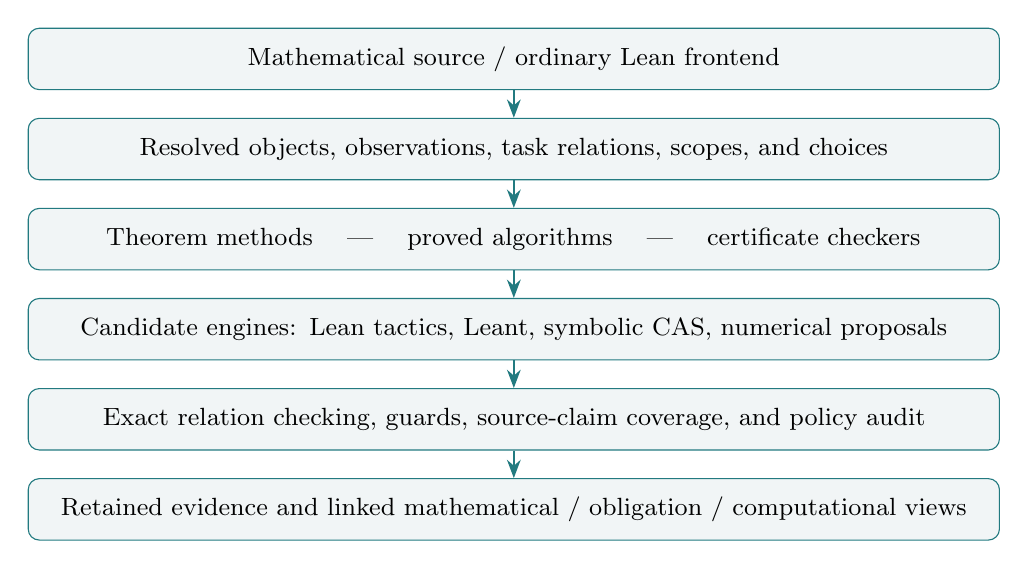
\begin{tikzpicture}[node distance=.35cm,
 box/.style={draw=accent,rounded corners,fill=pale,text width=12.1cm,
 align=center,minimum height=.78cm,font=\small},>={Stealth}]
\node[box] (a) {Mathematical source / ordinary Lean frontend};
\node[box,below=of a] (b) {Resolved objects, observations, task relations, scopes, and choices};
\node[box,below=of b] (c) {Theorem methods \quad | \quad proved algorithms \quad | \quad certificate checkers};
\node[box,below=of c] (d) {Candidate engines: Lean tactics, Leant, symbolic CAS, numerical proposals};
\node[box,below=of d] (e) {Exact relation checking, guards, source-claim coverage, and policy audit};
\node[box,below=of e] (f) {Retained evidence and linked mathematical / obligation / computational views};
\foreach \x/\y in {a/b,b/c,c/d,d/e,e/f} \draw[->,thick,accent] (\x)--(\y);
\end{tikzpicture}
\end{center}
The arrows describe information flow, not a claim that every stage is already
implemented. Candidate generation may be interactive and iterative; authority
enters only through the exact checked relation.

\subsection{Proved algorithms need justified executions}
Suppose Lean contains a proved normalizer \(f\) with
\(\forall e,\ \sem e=\sem{f(e)}\). Applying that theorem yields an equality with
\(f(e)\). If an external native execution returns a concrete \(n\), the application
does not yet establish \(n=f(e)\). That additional link needs kernel reduction,
a checked execution certificate, or an explicitly stronger execution trust policy.

Thus there are two preferred publication paths. A small enough verified algorithm
can run by kernel-justified computation. A faster producer can instead emit a
certificate whose independently checked correctness relates the original input
to the returned output. The producer can be optimized, replaced, or even
unverified without changing the logical acceptance rule.

The default Accord publication profile should not rely on undisclosed native
computation axioms. An optional accelerated profile may permit them, but its
receipt must say what it trusts. Current Lean documentation explains that native
computation increases the trusted base and, since Lean 4.29, uses dedicated
per-computation axioms rather than only the historical \code{Lean.trustCompiler}
constant\cite{leanvalidation}. A blacklist of that one name is therefore not an
adequate trust policy.

This is why ``a CAS based on verified algorithms'' should mean both verified
mathematical algorithms and an honest account of their executions. Merely
implementing an algorithm in Lean, or proving an unrelated reference version,
is not enough.

\subsection{A small semantic core, optimized certified representations}
The long-term core should contain proved operations on exact integers and
rationals, polynomial representations, finite sums, truncated formal series,
and elementary interval bounds. Optimized implementations can use sparse maps,
dense arrays, modular arithmetic, or native libraries, provided their output is
related to the semantic model by checked refinement or certificates.

This separates three maintenance tasks: the mathematical theorem, the representation
correctness proof, and the performance implementation. A new sparse multiplication
algorithm need not change every user's polynomial theorem. Conversely, a change
from characteristic zero to arbitrary characteristic changes the semantic contract
and cannot be treated as a backend optimization.

A minimal first release need not implement factorization, root isolation, real
quantifier elimination, integration, and special functions simultaneously. It
should publish a capability table with exact domains and failure behavior. Larger
algorithms can join only when their certificates and guards are equally explicit.

\subsection{Polynomial certificates: inexpensive claims before expensive completeness}
A useful initial certificate format is
\[
 g=\sum_{i=1}^{m}q_i f_i
\]
in a declared polynomial ring. A coefficient-normalization checker verifies this
identity. If the hypotheses say \(f_i(x)=0\), it follows that \(g(x)=0\).
For instance,
\[
 X^3-X=(X+1)(X^2-X)
\]
certifies that \(x^2=x\) implies \(x^3=x\). The producer need not be a verified
Gr\"obner-basis implementation for this one implication to be sound.

The limits are crucial. A certificate that one polynomial belongs to an ideal
is not a complete ideal-membership decision procedure. To claim that a transformed
system has the same ideal, both inclusions need evidence. To claim a complete
normal-form test, one also needs the applicable basis criterion, coefficient-domain
assumptions, and monomial-order conditions. To derive inconsistency from a
certificate for \(1\), the ambient interpretation must satisfy \(1\ne0\).
To infer \(p=0\) from \(p^k=0\), the selected domain must justify eliminating
nilpotents; this inference is false in a general commutative rational algebra.

These distinctions should appear in result types. A command requesting a
\emph{complete factorization} needs multiplication correctness and irreducibility
claims; a command requesting a \emph{factorization} may need only multiplication
correctness. A square-free decomposition has still another specification.

A relevant maintenance warning comes from current Mathlib documentation:
\code{polyrith} is marked unsupported because its external Sage service became
unavailable; the documentation points to \code{grobner} for polynomial reasoning
but distinguishes it from a \code{linear_combination} suggestion workflow
\cite{polyrith}. The architectural lesson is not to depend on a public CAS service
for replay, nor to equate two tactics' interface guarantees merely because both
can solve polynomial goals.

\subsection{Algebraic numbers and radicals need a root identity}
An exact real algebraic number can be represented by a polynomial and a rational
isolating interval, with evidence of existence and uniqueness of a root in that
interval. The polynomial alone does not identify which root is meant. Two
representations can be compared through a proved common root characterization;
a printed decimal is not their semantic identity.

For radical denesting, a producer may guess an expression \(u\), but the checker
must verify both the algebraic relation and the selected branch. For example,
\[
 (1+\sqrt2)^2=3+2\sqrt2,\qquad 1+\sqrt2\ge0
\]
identifies the principal nonnegative root, hence
\(\sqrt{3+2\sqrt2}=1+\sqrt2\). Squaring alone would also accept the negative
of the proposed expression. Similarly, \(\sqrt{x^2}=|x|\), not unconditionally
\(x\). A positive-branch shortcut owes \(x\ge0\).

Complex algebraic computations need an equally explicit root identity or branch
specification. No default rewriter should turn a formally valid polynomial relation
into an identity of chosen analytic branches. Root isolation and branch reasoning
are plausible verified-CAS modules, not features this article claims to have
implemented.

\subsection{Symbolic summation and differential equations are certificate tasks}
For finite summation, an antidifference candidate \(G\) is useful when the checker
establishes \(f(k)=G(k+1)-G(k)\) on every required index. Telescoping then gives the
sum, including its boundary terms. A rational certificate may introduce denominator
guards at specific indices; clearing them generically does not validate endpoint
substitution. An infinite sum additionally requires the appropriate limiting or
summability theorem.

For a recurrence or differential equation, a candidate closed form can be checked
against the equation and initial or boundary data. Uniqueness is a separate theorem.
A recurrence whose leading coefficient vanishes at a parameter value may require
extra initial data or a separate branch. A CAS output that passes several initial
values is not a universal solution certificate.

This is a useful division of labor: discovery can use sophisticated heuristic
algorithms; verification asks for a relation that is smaller, local, and exact.
When no compact complete certificate is known for the selected problem, the
system can return a weaker checked claim or remain unresolved, but cannot relabel
it as complete.

\subsection{Prior work establishes feasibility, not ready-made integration}
Structured mathematical proof is established prior art; Isar explicitly combines
structured readable proof with semi-automated reasoning\cite{isar}. Lean's own
pipeline separates extensible elaboration from kernel checking and exposes
source-linked elaboration metadata\cite{leanelab}. Accord's contribution is not
that separation but the relation-specific computational interface built above it.

Verified symbolic algorithms also have substantial precedents. Cohen and Mahboubi
formalize algebraic real-closed-field theory and quantifier elimination in Coq
\cite{cohenmahboubi}. Kosaian, Tan, and Platzer give a complete real quantifier
elimination algorithm in Isabelle/HOL\cite{kosaian}. These works support the
feasibility of formally verified decision procedures while also illustrating how
substantial the algebraic infrastructure can be. They are not evidence that an
efficient general-purpose Lean CAS is already available.

The Interval package for Rocq provides proof automation for real inequalities
using interval-style bounds and supports explicit bounding hypotheses for
unrecognized subexpressions\cite{interval}. It is a particularly relevant
precedent for distinguishing a proved enclosure from an unverified floating-point
answer. Porting ideas is not the same as transporting their proofs across kernels;
Accord still needs Lean-checked implementations or a justified interoperability
mechanism.

\section{Guards and completeness: the first computational example}\label{sec:linear}
\subsection{A complete answer to a small equation}
Over \(\R\), consider the parameterized task \(ax=b\). The complete answer is
\[
 S(a,b)=
 \begin{cases}
 \{b/a\},&a\ne0,\\
 \R,&a=0\text{ and }b=0,\\
 \varnothing,&a=0\text{ and }b\ne0.
 \end{cases}
\]

\begin{proposition}
For all real \(a,b,x\), \(ax=b\) if and only if \(x\in S(a,b)\).
\end{proposition}
\begin{proof}
If \(a\ne0\), multiplying \(ax=b\) by \(a^{-1}\) gives \(x=b/a\), and substituting
\(x=b/a\) gives \(ax=b\). If \(a=0\), the equation reduces to \(0=b\), independently
of \(x\). It is therefore true for every \(x\) when \(b=0\), and false for every
\(x\) when \(b\ne0\). The cases are exhaustive and disjoint.
\end{proof}

The output object is a set described by cases, not necessarily a finite list.
Representing every solution request by \code{List Real} would already make the
\(a=b=0\) case impossible to describe faithfully. Infinite solution families and
parameters are part of the data model, not exceptional error strings.

\subsection{The exact obligation record}
The nonzero branch owes a proof that division by \(a\) preserves equivalence.
The zero branch owes the simplification \(ax=0\). The case-split node owes
coverage. If the implementation promises disjoint branch selection, it also
records disjointness; ordinary logical case analysis alone does not require a
canonical disjoint output format.

A minimal mathematical receipt is:
\begin{lstlisting}
task:       solve-completely
predicate:  fun x : Real => a*x = b
output:     S(a,b)
guards:     discharged inside recorded parameter branches
soundness:  forall x, x in S(a,b) -> a*x = b
coverage:   forall x, a*x = b -> x in S(a,b)
origin:     exact parameters, context, statement, environment
\end{lstlisting}
The two implications can be stored separately for inspection, but both are needed
for this task. When only one exists, the UI must label the result accordingly.

\subsection{Why specialization is a semantic operation}
The generic expression \(b/a\) cannot be specialized to \(a=0\) while retaining its
nonzero-branch theorem. Likewise,
\[
 \frac{x^2-1}{x-1}=x+1
\]
is valid for real \(x\ne1\). Under Lean's total real division convention, at \(x=1\)
the left side is \(0\) and the right side is \(2\). The identity of rational
functions is a different statement: evaluating that identity at a pole is not
licensed by equality in the rational-function field.

\begin{proposition}[Guarded specialization]
Suppose a checked transformation is quantified over parameters \(a\) and has type
\(\forall a,\ G(a)\to R(a,e(a),e'(a))\). At a parameter value \(a_0\), the same
transformation establishes the desired instance when evidence of \(G(a_0)\) is
supplied. The quantified conditional theorem alone does not establish the
unguarded instance.
\end{proposition}
\begin{proof}
Instantiate the theorem at \(a_0\), then apply it to the guard proof. Without the
second application the result has implication type, not the desired conclusion.
\end{proof}

The implementation consequence is useful: retain generic results with their
parameter guards and specialize them through the same checked interface. There
is no need to discard every computation near a degenerate parameter; there is a
need to refuse invalid transport of its guarantee.

\subsection{A negative neighbor that exposes lost solutions}
Starting from \(x^2=x\), division by \(x\) yields \(x=1\) only in the branch
\(x\ne0\). The original equation also has the solution \(x=0\). A solver returning
\(\{1\}\) passes a witness-validity check and fails the requested all-solution
check. The exact counterexample is small and can itself be checked.

This example is an excellent first integration test because it distinguishes
three superficially similar implementations: one that blindly divides, one that
proves its returned witness, and one that actually solves completely. Only the
third satisfies the authored request.

\section{Finite algebra without losing generality}\label{sec:binomial}
\subsection{The mathematical move in the source}
The inspected binomial module proves, for natural \(n,j\), the integer identity
\[
 \sum_{k=j}^{n}(-1)^{n-k}\binom nk\binom kj=[n=j],
\]
where an empty interval contributes zero and \([P]\) is the integer indicator.
Its implementation splits the empty case, reindexes an interval, applies the
binomial product identity, transports casts, and invokes an alternating-row
identity\cite{pbinomial}.

For \(j\le n\), write \(n=j+m\). The bijection \(i\mapsto j+i\) from
\(0\le i\le m\) to \(j\le k\le n\), together with
\[
 \binom n{j+i}\binom{j+i}j=\binom nj\binom mi,
\]
gives
\[
 \sum_{k=j}^{n}(-1)^{n-k}\binom nk\binom kj
 =\binom nj\sum_{i=0}^{m}(-1)^{m-i}\binom mi
 =\binom nj[m=0]=[n=j].
\]
For \(n<j\), both the empty sum and the indicator are zero.

An Accord source can retain exactly these choices:
\begin{lstlisting}
case n < j:
  conclude by empty_interval
case j <= n:
  write n = j+m with m : Nat
  reindex by i |-> j+i from [0..m] to [j..n]
  transform summands by binomial_product
  calculate using alternating_binomial_row
\end{lstlisting}
The notation \code{[0..m]} has an explicitly inclusive natural-number meaning in
this profile. It is not resolved by trying interval conventions until a proof
succeeds.

\subsection{What the CAS does, and what it does not do}
The finite-index method generates membership, injectivity, coverage, and summand
correspondence obligations. A small arithmetic profile can often solve the bounds.
A polynomial normalizer can handle the rearrangements of integer factors. It does
not invent the map \(i\mapsto j+i\) invisibly as a change in the author's stated
method, and it does not treat the arbitrary natural bound as a finite numeral to
be exhaustively evaluated.

Replacing the target interval by \([0,m)\) loses an endpoint. The method should
report failure of coverage at that endpoint. It should not retain the word
``reindex'' while allowing an unrelated prover to close the final equality.
Replacing a finite sum by a conditionally convergent infinite series is also not
a variant of the same certificate.

\subsection{The transform theorem remains module-valued}
Let \(M\) be an additive commutative group. Integer kernels act on \(M\) by repeated
addition and negation. Consequently the orthogonality identity proves that
\[
 b_n=\sum_{k=0}^{n}\binom nk\,a_k
 \quad\Longleftrightarrow\quad
 a_n=\sum_{k=0}^{n}(-1)^{n-k}\binom nk\,b_k,
\]
with coefficients interpreted as integer scalar actions, without multiplying two
elements of \(M\). Accord should perform the kernel calculation in \(\Z\), then
apply the existing triangular-transform interface at the original module type.
The inspected source already does this\cite{pbinomial}.

This is a control against exaggerated language claims. The public transform
result is already short because a good mathematical abstraction exists. The new
system earns its place only if it reduces the cost of authoring, locating,
explaining, or maintaining the supporting orthogonality step. Its library and
normalization rules must also be available to the ordinary Lean baseline.

\section{Formal series as a native computational domain}\label{sec:series}
\subsection{The Abel example is more than an algebra exercise}
Let \(A\) be a commutative \(\Q\)-algebra and let \(\iota:\Q\to A\) denote its
structure map. Define the formal exponential with parameter \(c\in A\) by
\[
 E_c(t)=\sum_{n\ge0}\iota(1/n!)c^nt^n.
\]
Suppose \(T\in A[\![ t]\!]\) satisfies
\begin{equation}\label{eq:abel}
 T=tE_{-a}(T).
\end{equation}
The inspected Abel module proves the coefficient formula for every such \(T\),
not just for its constructed canonical solution\cite{pabel}.

This is a demanding interface test. Formal substitution must be admissible.
The coefficients include rational scalars but \(A\) need not be a field.
The zero coefficient differs from the positive-degree pattern. The theorem is
uniform in the degree, not the result of computing a finite table. Each distinction
should survive the shortened source.

\subsection{A complete derivation of the coefficient calculation}
Taking constant coefficients in \eqref{eq:abel} gives \(T(0)=0\); here \(T(0)\)
means the constant coefficient, not an assertion about analytic evaluation.
Substitution of \(T\) into arbitrary formal series is therefore admissible by the
zero-constant-term criterion.

Use the formal Lagrange--B\"urmann coefficient theorem in the form applied by the
ProveIt module\cite{pabel}. For positive integer \(N\), outer series \(F\), and
\(T=t\phi(T)\), its coefficient relation is
\begin{equation}\label{eq:lagrange}
 N_A\,\coeff tN F(T)=\coeff u{N-1}\bigl(F'(u)\phi(u)^N\bigr),
\end{equation}
under the requisite substitution and inversion hypotheses, where \(N_A=\iota(N)\).
Here \(\phi=E_{-a}\) is a unit with inverse \(E_a\), so those multiplicative
inversion premises have explicit witnesses.

Take \(F=E_x\). The formal identities \(E_x'=xE_x\),
\(E_cE_d=E_{c+d}\), and \(E_c^N=E_{Nc}\) give
\[
 F'(u)\phi(u)^N=xE_{x-Na}(u).
\]
Its degree-\(N-1\) coefficient is
\[
 x(x-Na)^{N-1}\iota\!\left(\frac1{(N-1)!}\right).
\]
Since \(N>0\), the element \(N_A\) has the displayed inverse \(\iota(1/N)\):
\[
 \iota(1/N)N_A=\iota((1/N)N)=1.
\]
Multiplying \eqref{eq:lagrange} by that inverse yields
\begin{equation}\label{eq:abelcoeff}
 \coeff tN E_x(T)
 =\iota\!\left(\frac1{N!}\right)x(x-Na)^{N-1},\qquad N\ge1.
\end{equation}
The constant coefficient is \(1\), because \(T(0)=0\). Equivalently,
\[
 E_x(T)=\sum_{n\ge0}\iota(1/n!)A_n(a,x)t^n,
 \quad A_0(a,x)=1,\quad A_{n+1}(a,x)=x\bigl(x-(n+1)a\bigr)^n.
\]

No cancellation of a merely nonzero element of \(A\) has occurred. The proof uses
an explicit unit, the image of a nonzero rational number. It does not require
injectivity of \(\iota\), nor does it exclude the trivial algebra. The distinction
between \emph{nonzero} and \emph{invertible} is indispensable in general rings.

\subsection{The proposed source and its generated obligations}
\begin{lstlisting}
context A : commutative Q-algebra
context a x : A
context T : formal series over A
assume hT : T = t * E(-a)(T)

claim coefficients:
  coefficient 0 of E(x)(T) = 1
  forall n : Nat, coefficient (n+1) of E(x)(T)
    = rational_scalar(1/(n+1)!) * x*(x-(n+1)*a)^n
proof
  derive constant_coefficient T = 0 from hT
  at positive degree N:
    transform coefficient by Lagrange_Burmann using hT
    calculate formal derivative and exponential product
    cancel N using rational_unit N
  at degree 0:
    calculate constant coefficient
\end{lstlisting}

The field-like visual notation is a renderer for multiplication by
\(\iota(1/(n+1)!)\), not an instruction to synthesize a field structure on \(A\).
The interface shows this interpretation once in the definition package and again
on demand at the expression. The obligations include substitution admissibility,
the unit equation, positive degree, and the applicability of the specific
Lagrange theorem. Their routine proofs can be hidden, but their propositions
remain accessible.

The key mathematical decision is Lagrange inversion. Formal differentiation,
exponential multiplication, and rational-scalar normalization are natural verified
CAS operations. They should be shared library components, not a purpose-built
``prove the Abel theorem'' oracle. A held-out exponential coefficient family must
reuse them before their apparent compression is credited as infrastructure value.

\subsection{Definition-side compression through observations}
An exponential generating function package can provide
\[
 \operatorname{egf}(a)_n=\iota(1/n!)a_n
\]
as its coefficient observation theorem, together with proved addition,
product/binomial-convolution, and scalar-action interfaces. Users can reason about
sequences without repeating \code{coeff}, \code{algebraMap}, factorial, and
range-conversion plumbing at every step.

There is a design choice here: the semantic anchor can be the formal series with
coefficient observations, or the sequence with its EGF representation. Both are
valid. The first experiment should implement both in ordinary Lean, charge their
bridge-lemma costs, and compare downstream proofs. The new surface cannot make
that library experiment unnecessary.

\subsection{Finite jets need a precision calculus}\label{sec:precision}
For \(N\ge1\), write
\[
 f\equiv_N g\quad\Longleftrightarrow\quad
 \forall n<N,\ \coeff Xn f=\coeff Xn g.
\]
Equivalently, \(f-g\) is divisible by \(X^N\). Over a commutative ring, the following
rules give a small useful precision calculus:
\begin{align*}
 f\equiv_N g,\quad h\equiv_M k
 &\ \Longrightarrow\ f+h\equiv_{\min(N,M)}g+k,\\
 f\equiv_N g,\quad h\equiv_M k
 &\ \Longrightarrow\ fh\equiv_{\min(N,M)}gk,\\
 f\equiv_N g
 &\ \Longrightarrow\ f'\equiv_{N-1}g'.
\end{align*}
The paired premises are conjunctive. At precision zero the conclusion imposes no
coefficient conditions.

For the derivative rule, write \(f-g=X^Nu\). Then
\[
 f'-g'=NX^{N-1}u+X^Nu',
\]
which is divisible by \(X^{N-1}\). In particular, differentiating a representative
of a jet modulo \(X^N\) does \emph{not} automatically define its derivative modulo
\(X^N\); it is well defined at one less order.

If the constant coefficient is a unit, multiplicative inversion preserves
precision. Indeed, for invertible \(f,g\),
\(f^{-1}-g^{-1}=f^{-1}(g-f)g^{-1}\), so divisibility by \(X^N\) is retained.
The unit hypothesis belongs to the computational contract.

\begin{proposition}[A sufficient composition-precision rule]
Let \(N,M,r\ge1\). Suppose \(f\equiv_N\widetilde f\),
\(g\equiv_M\widetilde g\), both inner series have constant coefficient zero,
and \(g\) is divisible by \(X^r\). Then
\[
 f(g)\equiv_{\min(rN,M)}\widetilde f(\widetilde g).
\]
\end{proposition}
\begin{proof}
Write \(f-\widetilde f=X^Nh\). Substitution into \(g\) gives
\(f(g)-\widetilde f(g)=g^Nh(g)\), which is divisible by \(X^{rN}\).
For the other difference use, term by term,
\[
 g^k-\widetilde g^{\,k}
 =(g-\widetilde g)\sum_{i=0}^{k-1}g^i\widetilde g^{\,k-1-i}.
\]
Because both inner constant coefficients vanish, the resulting infinite series
is coefficientwise well defined: each fixed coefficient receives contributions
from only finitely many powers. Thus
\(\widetilde f(g)-\widetilde f(\widetilde g)\) is divisible by \(X^M\).
Adding the differences proves the stated minimum bound.
\end{proof}

This rule is sufficient, not optimal in every example. Extra vanishing or nilpotence
may improve precision. A more sophisticated backend can provide a stronger proved
bound, but cannot claim it merely from observed zero coefficients.

\subsection{Exploration can generate a conjecture, not a universal receipt}
Computing \(T\) and \(E_x(T)\) modulo \(t^{10}\) is an appropriate exploratory CAS
operation. It can suggest \eqref{eq:abelcoeff}; it does not prove that formula for
arbitrary degree. The universal result needs a symbolic theorem such as the
Lagrange derivation above or a proved recurrence with enough initial data.

The finite approximation itself has a simple structural explanation. Starting
from \(T_0=0\), iterate
\(T_{k+1}=tE_{-a}(T_k)\). Two zero-constant-term series that agree modulo \(t^m\)
have images under this map agreeing modulo \(t^{m+1}\). Hence each iteration fixes
one more coefficient. Coefficientwise stabilization constructs the formal
solution; no analytic convergence theorem is involved. The same argument shows
uniqueness by improving agreement one order at a time.

The companion computes ten coefficients for nineteen parameter pairs, including
three in \(\Q[\epsilon]/(\epsilon^2)\). This non-field algebra is a useful control
against an accidentally field-only implementation. The finite checks agree with
\eqref{eq:abelcoeff}, but the universal algebraic claim rests on the mathematical
derivation, not on the test table.

\section{Local calculus with symbolic derivative computation}\label{sec:calculus}
\subsection{Preserve the theorem's exact local assumptions}
Let \(U\subseteq\R\) be open, and let \(W,\phi:\R\to\R\). Suppose that at each
\(x\in U\), \(W\) has derivative \(\phi(W(x))\). Let \(G_n,G_n':\R\to\R\) satisfy
\[
 G_0(W(x))=W(x),\qquad
 G_{n+1}(W(x))=G_n'(W(x))\phi(W(x)),
\]
and suppose \(G_n\) has derivative \(G_n'(W(x))\) at the reached value \(W(x)\).
The inspected theorem proves
\begin{equation}\label{eq:autonomous}
 W^{(n)}(x)=G_n(W(x)),\qquad x\in U.
\end{equation}
It does not require the auxiliary derivatives away from the reached values
\cite{pode}.

The proof is induction on \(n\). The base is the given identity for \(G_0\). In the
successor case, the induction identity holds on \(U\), hence in a neighborhood of
the chosen \(x\). Transfer differentiation across that neighborhood equality;
then the chain rule gives
\[
 W^{(n+1)}(x)=G_n'(W(x))W'(x)
 =G_n'(W(x))\phi(W(x))=G_{n+1}(W(x)).
\]
This is the whole mathematical argument. The neighborhood equality is not an
optional implementation detail: \(f(t)=0\) and \(g(t)=t\) agree at zero but have
different derivatives there.

\subsection{Locality as a capability with a proof}
The proposed source makes the induction scope and differentiation locality explicit:
\begin{lstlisting}
induct n retaining the identity on U
case successor:
  at x in U:
    use neighborhood U at x, justified by openness
    differentiate the induction identity near x
    calculate by chain_rule using hW, hGd, hGs
\end{lstlisting}

Internally, the open-set membership theorem supplies a neighborhood certificate;
the identity on \(U\) supplies an eventual equality. A composite ordinary Lean
wrapper can implement this move. It should expose the neighborhood and derivative
premises as named roles while leaving their actual propositions unchanged.

A locality block is not permission to assume continuity, differentiability, or
nonvanishing. It is a scoped context that records where the available facts hold.
Equality at a point, equality on a set, equality of germs, and equality of formal
series are distinct relations. No amount of successful algebraic normalization
can change one into another without a transport theorem.

\subsection{A CAS specialization: Lambert derivative polynomials}
Now consider a solution of
\[
 W'(x)=\frac{e^{-W(x)}}{1+W(x)}
\]
on an open domain where \(W(x)\ne-1\). This is the autonomous derivative form
discussed in the source's Lambert example\cite{pode}. The pole-avoidance condition
is explicitly part of this specialization; it is not added to the general theorem.

Define \(P_1(w)=1\) and, for \(n\ge1\),
\begin{equation}\label{eq:lambertpoly}
 P_{n+1}(w)=(1+w)P_n'(w)-(nw+3n-1)P_n(w).
\end{equation}
Put
\[
 H_n(w)=\frac{e^{-nw}P_n(w)}{(1+w)^{2n-1}},\qquad n\ge1.
\]
At \(w\ne-1\), ordinary product and quotient differentiation gives
\[
 H_n'(w)=\frac{e^{-nw}}{(1+w)^{2n}}
 \left((1+w)P_n'(w)-\bigl(n(1+w)+2n-1\bigr)P_n(w)\right).
\]
Multiplying by \(e^{-w}/(1+w)\) produces
\[
 H_n'(w)\frac{e^{-w}}{1+w}
 =\frac{e^{-(n+1)w}P_{n+1}(w)}{(1+w)^{2n+1}}
 =H_{n+1}(w).
\]
With \(G_0(w)=w\) and \(G_n=H_n\) for \(n\ge1\), the local-calculus theorem
therefore yields the corresponding higher-derivative formula.

This is an attractive division of labor. The mathematician chooses the
factorization \(e^{-nw}(1+w)^{-(2n-1)}P_n(w)\), which reveals a polynomial
recurrence. The symbolic engine differentiates that expression under a recorded
nonzero guard and certifies the normalized numerator. Leant can reconstruct the
applications and local premise passing. Neither component needs to discover or
silently strengthen the global analytic theorem.

The first polynomials are
\begin{align*}
 P_1(w)&=1,\\
 P_2(w)&=-w-2,\\
 P_3(w)&=2w^2+8w+9,\\
 P_4(w)&=-6w^3-36w^2-79w-64.
\end{align*}
The companion checks the polynomial numerator calculation through the transition
to \(P_6\). These checks do not certify the real differentiation theorem; that
requires the derivative lemmas and the pole guard. They illustrate the small exact
algebraic certificate that can sit inside the larger analytic proof.

\subsection{What remains visible to the reader}
The factorization ansatz, the recurrence, the domain avoiding the pole, and the
local induction remain visible. The reader can expand the rational derivative
normalization, but it need not occupy the main page. Removing the pole condition
should lead to a failed method guard, not to a solver quietly proving a different
totalized formula.

This example also demonstrates why minimizing proof length alone is inadequate.
A one-line invocation of the already proved derivative theorem may be excellent
for a specialist. A short derivation exposing the polynomial recurrence may be
better for a reader learning the mathematics. Both should be views of the same
accepted material, not competing notions of correctness.

\section{Certified numerical computation without replacing the object}\label{sec:numerical}
Let \(p(x)=x^3-x-1\). On \([1,3/2]\),
\[
 p(1)=-1,\qquad p(3/2)=7/8,\qquad p'(x)=3x^2-1\ge2.
\]
Continuity and the intermediate value theorem give a root in the interval.
The derivative bound makes \(p\) strictly increasing there, so the root is unique
in that interval. Denote this uniquely specified root by \(r\). No claim about
all roots outside the interval is needed for this task.

A rational bisection producer returns endpoints and exact sign evidence. The
companion, after twenty bisections, returns
\begin{equation}\label{eq:bracket}
 \frac{1389067}{1048576}<r<\frac{2778135}{2097152},
 \qquad u-l=\frac1{2097152}.
\end{equation}
The strict endpoint signs, containment in the original interval, and uniqueness
identify the same \(r\) throughout refinement. The output is not a newly chosen
root and not an assertion that \(r\) equals a printed decimal.

A second certificate format uses a rational approximation \(q\in[1,3/2]\).
The mean value theorem and \(p'\ge2\) show
\begin{equation}\label{eq:residual}
 |r-q|\le\frac{|p(q)|}{2}.
\end{equation}
Indeed, when \(r\ne q\), the mean value theorem gives
\(p(q)-p(r)=p'(\xi)(q-r)\) for an intermediate \(\xi\), and taking absolute values
proves the bound; the case \(r=q\) is immediate. The residual \(p(q)\) is an exact
rational computation. A numerical engine can choose \(q\) by any heuristic,
provided the certificate checks the required interval and residual claims.

The two certificates serve different interactions. Bisection provides nested
intervals and a predictable width. A residual estimate can certify a very good
proposal without replaying the process that found it. Neither grants permission
to assert equality from closeness. A requested strict inequality involving \(r\)
can be concluded when the certified enclosure separates it from the boundary;
otherwise the result is unresolved and a narrower interval may be requested.

\decision{Approximation is a first-class relation with a budget and a proved
error bound. It is never an implicit coercion from an exact mathematical object
to a floating-point value.}

\section{Leant as the structural assembly and suggestion service}\label{sec:leant}
\subsection{What can be reused directly}
Leant's inspected verification module already makes a valuable distinction:
its nominal \code{Verified} wrapper records acceptance by a supplied callback,
not a kernel proof or behavioral certificate. The scheduler tries spellings of a
candidate in order, counts accepted groups toward a quota, and avoids forcing
additional candidates after the quota is satisfied\cite{lverification}.

Its engine retains typed candidate origins, provider bindings, renderer-related
information, and a distinction between candidates, qualified refutation, and
no-term outcomes\cite{lengine}. These are useful architectural assets. Accord
should reuse the Haskell engines through a narrow adapter rather than commission
a wholesale rewrite before measuring their value.

The first use case is structural assembly: apply an available theorem, instantiate
its binders, compose maps, project a conjunction, supply an induction hypothesis,
or assemble the premises of a CAS correctness theorem. A verified algebra
normalizer and Leant solve different problems and should remain separate providers.

\subsection{The request must be an exact scoped obligation}
The Lean-side adapter owns the actual expression and its ordered context. External
providers receive a versioned serialization or opaque handles for unsupported
atoms, together with an exact request identity. Pretty-printed text can aid search
and diagnosis but is not the authority used for final acceptance.

A candidate is re-elaborated or imported at the original target in the original
context, with no permission to invent implicit parameters that change its meaning.
A returned proof of a more convenient specialization is rejected. Provider-created
names are scoped to the candidate transaction. A late reply after an undo or source
edit is stale even if its printed target looks unchanged.

The allowed local premises, allowed library declarations, and transitive axiom
policy are three different restrictions. A declaration required to type a permitted
hypothesis does not thereby become an unrestricted mathematical premise. The
adapter must retain the dependency closure needed for well-typed contexts while
checking the intended proof-use policy separately.

\subsection{Negative outcomes need more than a soundness bit}
Leant's engine explicitly qualifies negative outcomes by both the search engine's
completeness claim and the translation's treatment of structure-hiding atoms
\cite{lengine}. This is a good operational discipline. It is not, by itself, a Lean
proof of the negation of the original theorem.

The second synthesis proposes generalizing the safety bit to a per-node abstraction
list\cite{review}. I would adopt the diagnostic list but not treat its emptiness
as a proof. An implementation can omit a relevant abstraction; an engine can
incorrectly claim completeness. For a certified negative result the language needs
either a proof of the original negation, a checked counterexample with the required
logical connection, or a checked completeness-and-adequacy argument for the exact
fragment.

For example, to transport uninhabitability from a search type \(F\) to an original
type \(T\), a sufficient bridge is a checked function \(T\to F\), together with
\(F\to\mathrm{False}\). Their composition proves \(T\to\mathrm{False}\).
An untrusted annotation ``translation lossless'' is not that bridge.

The provider's abstraction report is therefore separate from the proof ledger's
dependency record. The first explains search capability and lost information;
the second records actual typing and proof dependencies. A language model may
propose a counterexample, but only its checked mathematical evidence can become
a refutation. Timeout, cancellation, and exhausted candidates remain nonlogical
outcomes.

\subsection{A displayed suggestion must be the thing that was checked}
The inspected \code{suggestTactic} path probes an immutable proof-state identifier,
extracts possible \code{Try this} text, and classifies progress partly through a
reduced visible goal count. On the direct path, that extracted display text is not
independently replayed before it is offered\cite{lmain}. This is a specific
publication-boundary concern, not an allegation that the Lean kernel accepts
invalid mathematics.

Accord's adapter should retain four distinct states:
\begin{lstlisting}
ProbeAccepted(original_command, original_state, result_state)
EditReplayed(exact_displayed_source, original_state, result_state)
GoalProgress(closed_goal_ids, remaining_goal_ids)
DocumentSealed(exact_claim_evidence, assertion_coverage, policy)
\end{lstlisting}

To advertise an edit as verified, replay the exact displayed text from the same
origin in a disposable worker. To advertise a theorem as complete, inspect its
closed proof term, not only the visible goal count. To seal a document, also check
every asserted source claim. These statuses answer different questions and should
not share one green icon.

Per-probe heartbeats are useful, but the total interaction also needs a deadline,
candidate limit, memory policy, cancellation, and stale-origin rejection. Persistent
logical proof states do not isolate a process crash or arbitrary effects of a
metaprogram. Worker isolation protects the live session and the user's files;
subsequent proof checking protects logical acceptance.

\subsection{Data synthesis needs a specification, not just ranking}
For a proof hole of fixed proposition \(P\), any allowed checked proof is enough.
For a data hole of type \(A\to A\to A\), both projections inhabit the type.
A structural rank cannot decide which one the user intended. A finite test can
reject some candidates, but only proves the particular tested proposition.

During exploration, expose several accepted candidates together with the exact
properties checked. For publication, retain the selected object and its required
specification. Rejected alternatives belong in an optional exploration history,
not by default in the main mathematical article. If a property characterizes the
object only up to an equivalence, replacing it requires a proved transport
interface for the downstream observations; type inhabitation alone does not
license replacement.

This policy respects Leant's candidate-oriented interaction while avoiding a
published proof whose mathematical object depends on whichever candidate ranked
first after an engine update.

\section{From an exploratory notebook to an accepted document}\label{sec:lifecycle}
\subsection{Resolve meaning without pretending elaboration is one pass}
A statement seal should be understood as a boundary before untrusted discovery
can affect meaning, not as a requirement that every Lean elaboration task finishes
in one sequential pass. Lean's elaboration and macro expansion are interleaved,
and its information trees relate elaboration results to source syntax
\cite{leanelab}. Accord should work with that machinery rather than replace it with
an inaccurate pipeline model.

A node begins as a draft. Resolution fixes its expressions, binders, observations,
structures, and requested relation. Proof holes may remain, but unresolved choices
that would change the task are not exported as ordinary proof-search holes.
Construction tasks explicitly permit a result object to be proposed; their
specification is fixed first and their chosen result is retained upon acceptance.

Several obligations can share a metavariable. The scheduler must solve or commit
such connected constraints transactionally. A graph of source dependencies alone
is not sufficient to justify independent parallel mutation of shared elaboration
state. Once the exact obligations are closed over their contexts, workers can
attempt them independently and return candidates for validation.

\subsection{The fact index is scoped and evidence-aware}
A local index can classify facts by roles such as nonzero, positive, membership,
unit, differentiability, eventual equality, or coefficient identity. This helps
method applicability and Leant premise selection without making the index a
second logic. Every entry points to the actual proposition and its evidence.

Branch-local facts remain branch-local. Pending guards remain conditional.
A proof of \(x>0\) can justify \(x\ne0\) through a theorem; a heuristic tag
``probably positive'' cannot. When a branch context is inconsistent, arbitrary
propositions may be logically derivable, but the explanatory view should make any
explicit contradiction used visible rather than pretending an algebraic method
succeeded meaningfully. Detecting all inconsistent contexts is not promised.

Human references such as ``the previous inequality'' are stored as resolved node
references. A formatter may regenerate that phrase only when it still names the
same assertion. Inserting a new inequality must not silently retarget an accepted
proof. This is particularly important in a mathematical document with several
successive approximations of the same object.

\subsection{A semantic display that reveals the right differences}
The primary display should reveal domains, quantifier dependence, chosen structures,
branch conventions, index endpoints, and approximation order. It should not require
a mathematician to approve a raw serialized expression. A change from
\(\forall\varepsilon>0\,\exists\delta>0\) to one \(\delta\) valid for all
\(\varepsilon\), or from a formal series to an analytic function, must be visible
as a semantic change even when much of the notation remains similar.

The first round correctly distinguishes \emph{notices} from \emph{obligations}
\cite{synthesis,review}. ``This is natural truncated subtraction'' is a notice.
``This transport requires \(b\le a\)'' is an obligation. A notice can be acknowledged;
an obligation needs a proof. Acknowledgments are attached to the relevant resolved
expression and convention. A project can set a display convention, but it cannot
globally dismiss mathematical premises.

The deterministic mathematical rendering should be generated from typed nodes
and registered templates. Extra free prose is clearly commentary. The system
certifies its formal assertion nodes and their relations; it does not claim that
every informal sentence or unparsed formula in a notebook has been verified.
This prevents an attractive narrative from becoming a false second source of
mathematical authority.

\subsection{Visible choices, collapsed consequences}
The main article view should show chosen branches, induction invariants, new
objects, representation changes with nontrivial guards, and substantial analytic
premises. It should usually collapse routine normalization evidence and elementary
bound derivations whose statements are already apparent from the context.

This is not a permanent judgment that, for example, positivity is always routine.
In a root-selection problem it may be the decisive mathematical choice. Visibility
is tied to the role in the current argument, and the reader can expand any node.
A useful comprehension test is whether a reader can locate the condition whose
removal invalidates the step, not whether the interface hides the greatest number
of obligations.

\section{Publication, replay, and repair}\label{sec:replay}
\subsection{The artifact and its authority}
A publication bundle should retain the resolved theorem, approved definitions,
all formal assertion nodes, accepted computational outputs, exact proof evidence,
method and checker identities, the transitive dependency and axiom inventory,
and the source-to-evidence map. Readable Lean source and the mathematical document
are valuable companion representations.

A hash identifies the content being checked; it is not evidence that the content
is true. Likewise, a success message in a JSON response does not authorize a proof.
The validator checks the evidence against the exact relation in its recorded
context. It also checks every formal assertion node, including unused ones.
Otherwise a trivial final theorem could conceal an unproved or false intermediate
claim in the published argument.

For untrusted generated code, candidate elaboration belongs in a sandbox, with
accepted terms exported for checking against a separately established statement.
Current Lean guidance distinguishes ordinary kernel acceptance from stronger
rechecking and challenge-comparison workflows\cite{leanvalidation}. Accord should
reuse appropriate existing validation infrastructure rather than market a ledger
file as a security boundary.

\subsection{Discovery-independent is not computation-free}
A certificate can be much cheaper to check than to discover, but checking may still
require substantial polynomial arithmetic, exact integer computation, or reduction.
``Replay without search'' means that no candidate discovery service, model, public
CAS endpoint, or changing theorem-search inventory is needed. It does not mean
that checking takes constant time or never evaluates an algorithm.

Retained tactic source alone is a weaker artifact: replaying it can re-execute
metaprograms and normalization. The syntheses' discussion of \code{says} usefully
illustrates the distinction between freezing a proposed text and independently
replaying that text or retaining its proof term\cite{synthesis,review}. Accord
should store text for editing, exact evidence for acceptance, and the computational
certificate when it assists inspection or regeneration.

Large evidence should support sharing through checked auxiliary declarations or
a term graph. Compression and caching must not erase the dependency closure.
An untrusted serialized graph needs format and reference validation before use.
A trusted library snapshot can be reused according to a stated validation policy;
an arbitrary imported binary is not a cross-version proof standard.

\subsection{Four classes of changes}
Adopt the first synthesis's distinction between evidence-only, plan, object, and
statement changes\cite{synthesis}. An evidence-only update changes how an identical
relation is proved, leaving accepted objects and meanings fixed. A plan change
alters the mathematical decomposition or method. An object change selects a
new witness or representation with observable consequences. A statement change
alters binders, assumptions, definitions, structures, or the claimed relation.

For Accord, refining a certified interval for the same root is ordinarily an
additional observation, not replacement of the root. Replacing an arbitrary root
with the positive root is an object change. Upgrading a witness result to a
complete solution set is a stronger task relation. Replacing precision \(N\) by
\(N+1\) is a new stronger observation, not a textual formatting change.

An environment upgrade invalidates compatibility assumptions until revalidated.
When old evidence no longer checks, the stored readable source and method record
can guide repair, but they do not overrule the checker. The repaired result gets a
new receipt. The old receipt remains valid only relative to its old pinned
environment; nothing here promises stable binary terms across Lean versions.

\section{A buildable implementation program}\label{sec:implementation}
\subsection{The first vertical slice}
The smallest informative prototype is not a large grammar. It is one end-to-end
path from a typed request to a retained, replayable result. Implement a claim record,
a relation tag backed by a Lean proposition, a simple theorem wrapper, and one
polynomial-combination checker. Prove the checker's soundness in Lean. Give ordinary
Lean access to all of it.

The first user task is the parameterized equation in Section~\ref{sec:linear}.
Its mutations test guard handling, solution completeness, set-valued outputs,
and branch coverage. A result with only \(x=b/a\) must not satisfy the all-parameter
request. A certificate containing a corrupted coefficient must fail independently
of the producer's report.

This slice should retain the exact evidence and replay with discovery disabled.
It does not need a cloud service, general natural-language parsing, or an elaborate
agent scheduler. The acceptance boundary must nevertheless be exact from the
start, so the prototype does not bake in a text-based authority that later stages
must replace.

\subsection{Second slice: locality and formal precision}
Add an ordinary theorem wrapper for transferring derivatives across a neighborhood
identity. Test the actual autonomous-derivative pattern and the pointwise-only
negative neighbor. Add a coefficient observation package, finite jets, and proved
precision rules for addition, multiplication, inversion, differentiation, and
zero-constant-term substitution.

Use the Abel example to test arbitrary \(\Q\)-algebra generality and separate finite
exploration from uniform proof. A finite coefficient computation must not complete
a universally quantified coefficient theorem. The derivative of a jet must not
retain its old precision automatically. These are semantic acceptance tests, not
only numerical regression tests.

\subsection{Third slice: Leant and competing providers}
Connect Leant through the exact obligation adapter. Run the same structural goals
with existing Lean automation and with Leant, separating single-theorem applications
from genuine compositions. This isolates where the adapter contributes value.
Before proactive suggestions are advertised as verified edits, implement exact
displayed-source replay, stale-origin checks, and separation of goal progress from
whole-document completion.

A second CAS producer can then emit the same polynomial or enclosure certificate
format. Swapping producers should not change what is accepted. Cancellation and
worker failure should not corrupt the live state. Successful results should remain
usable offline after the producer is removed.

\subsection{What should wait}
Broad theorem discovery, automatic extraction of reusable methods, arbitrary
natural-language interpretation, complete special-function integration, and global
coherence of arbitrary representation networks should wait for evidence from the
smaller system. They are research directions, not requirements for the first useful
release.

Verified root isolation, advanced polynomial algorithms, and symbolic summation
can be added incrementally as ordinary mathematical packages with explicit
certificates. Their scope should be chosen by measured user demand and
implementation cost, not by a checklist intended to resemble a commercial CAS.

\section{Evaluation that can reject the proposal}\label{sec:evaluation}
\subsection{Three treatments, with equal mathematical assets}
Use three treatments: current idiomatic Lean; refactored Lean with the proposed
methods, object interfaces, CAS checkers, and synthesis services; and the Accord
frontend with exactly those same assets. The first-to-second comparison measures
library and tooling gains. The second-to-third comparison measures the language's
incremental value. Mixing the two would make every helper lemma look like a syntax
breakthrough.

Test authoring separately from reading and repair. Authors should produce accepted
proofs, recover from failed methods, and handle changed assumptions. Readers should
identify the main idea, state the meaning of a computed result, locate a needed
guard, and distinguish a witness from a complete characterization. Randomize and
counterbalance task order, and record prior mathematical and Lean experience.

The initial families should include finite reindexing, rational-algebra coefficient
extraction, local differentiation, parameter-dependent solving, root enclosures,
structural proof assembly, and a short existing theorem as a negative control.
Hold out entire theorem families or modules before developing adapters. Remove the
target theorem, aliases, and downstream consequences from permitted discovery and
cached evidence.

\subsection{Metrics and cost accounting}
Measure successful authoring time, editing actions, failed attempts, end-to-end
latency, tail latency, checking cost, evidence size, and repair effort. Measure
comprehension by concrete questions rather than aesthetic preference alone.
Source length is a descriptive statistic, not the objective.

Record package development cost \(L\), per-example authoring cost \(A_i\), and
maintenance cost \(R_i\):
\[
 C(n)=L+\sum_{i=1}^{n}(A_i+R_i).
\]
Report the components and actual held-out reuse. A specialized adapter used once
cannot be amortized over hypothetical future theorems. Also record which failures
come from missing mathematics, unsupported representation, resource exhaustion,
and poor diagnostics; those call for different engineering responses.

The source audit in the second synthesis is a useful sampling aid, but an
elaboration-level instrument still needs carefully defined labels and manual
calibration\cite{review,synthesis}. Information trees do not directly measure
human effort, identify the conceptual step, or reconstruct all unsuccessful
attempts that preceded the saved proof. Interactive event logs are needed for the
last question, with the author's consent.

\subsection{Discriminating negative tests}
\begin{longtable}{@{}P{.37\textwidth}P{.56\textwidth}@{}}
\toprule
Mutation & Required distinction or rejection \\
\midrule
\endhead
Cancel \(a\) in \(ax=b\) with \(a=0\) possible & Retain the guard or split parameters;
do not publish a generic singleton as the full answer.\\
Return only \(1\) for \(x^2=x\) & Witness validity can pass; all-solution coverage
must fail at \(0\).\\
Replace a principal radical by its negative & The square equation can pass;
branch evidence must fail.\\
Remove the upper endpoint in reindexing & The bijection's coverage obligation
must fail, even if another proof could establish some final goal.\\
Use field cancellation in a rational algebra with nilpotents & Reject the
unavailable field or cancellation premise; do not strengthen the domain.\\
Promote ten matching coefficients to a series identity & Keep only the finite-jet
relation; the universal claim remains open.\\
Differentiate at unchanged jet precision & Require a stronger input certificate
or lower the output order.\\
Differentiate equality at one point & Require neighborhood equality; retain the
original statement.\\
Treat a floating approximation as exact & Demand a checked equality, not merely
a narrow interval.\\
Accept a stale suggestion after undo & Reject the mismatched origin, regardless
of similar printed text.\\
Accept a different displayed tactic than the one probed & Withhold edit-verification
status until exact replay succeeds.\\
Include a false unused assertion & Reject document completion even if the final
theorem has an independent proof.\\
Treat empty candidate search as refutation & Return a nonlogical no-result status
unless exact negative evidence is checked.\\
Import a new method with the same name & Preserve existing resolution; require
explicit conflict resolution for new uses.\\
\bottomrule
\end{longtable}

A system that refuses every operation would pass a naive rejection-only suite.
Each mutation must therefore have a positive neighbor and a useful expected
explanation. Correct failure includes identifying the missing proposition and its
source node. Failure of an advertised method need not mean the theorem is false.

\subsection{Go/no-go decisions}
Exact-target preservation, correct scope, honest completeness labels, and rejection
of the known invalid certificates are hard requirements. Numerical usability
thresholds should be selected after a pilot estimates realistic variance; this
article does not invent measured percentage improvements.

Ablate the new syntax, object interfaces, automatic guards, CAS support, Leant,
progressive disclosure, and retained evidence separately. If only object packages
and better lemmas improve authoring, retain them. If the new view helps readers but
not authors, ship it as a renderer. If checking costs dominate, optimize certificate
formats and representations before adding more discovery machinery. If a complete
CAS feature is too costly, offer its weaker explicitly specified operation rather
than mislabeling it.

\section{Executed exhibits and remaining uncertainty}\label{sec:exhibits}
The companion \code{certificate_exhibits.py} uses only the Python standard library,
exact rational arithmetic, and a small implementation of the dual-number algebra
\(\Q[\epsilon]/(\epsilon^2)\). Its final run completed 267 checks:

\begin{tabularx}{\textwidth}{@{}Y r@{}}
\toprule
Exhibit & Checks \\
\midrule
Polynomial identity certificate, four coefficient corruptions, and arity rejection & 6\\
Sample equivalences for the parameterized linear solver & 60\\
Abel coefficients through degree nine at nineteen parameter pairs & 190\\
Formal-exponential guard, non-field control, finite-jet/full-series distinction & 3\\
Lambert polynomial numerator transitions and an explicit \(P_3\) control & 6\\
Rational root bracket and rejection of a false initial bracket & 2\\
\midrule
Total & 267\\
\bottomrule
\end{tabularx}

The output file \code{exhibit_results.json} records the counts, polynomial
coefficients, rational enclosure, and Python version. The code does not implement
an Accord parser, a Lean adapter, a verified compiler, a full CAS, or a general
certificate security boundary. Its parameter tests are finite samples. Its
arithmetic checker is Python code, not a proved Lean checker. The mathematical
arguments in this article are paper proofs and specializations of cited
source theorems, not a new machine-checked formalization.

The useful role of these exhibits is narrower: they make some proposed certificate
objects concrete, exercise nearby failures, and separate the algebraic subproblem
from the larger analytic or universally quantified theorem. That is stronger than
an unexplained pseudocode promise, but substantially weaker than the integration
milestones specified above.

\section{Conclusion}
The opportunity is not another set of pleasant proof keywords. It is a mathematical
workbench that connects objects, computational representations, and proved
properties through explicit contracts.

Accord makes the decisive distinctions part of the task: equality or implication,
witness or complete solution set, finite jet or full series, pointwise or local
identity, approximation or exact object, proved algorithm or trusted execution.
The mathematician chooses the meaning; theorem libraries, verified algorithms,
certificate checkers, and Leant reconstruct its formal consequences.

Evaluate this proposal through a small shared implementation, preserved generality,
positive and negative neighboring examples, and measured benefit over equally
equipped Lean. A new authored language is one possible outcome. Better libraries,
certified computation, and a mathematical document view would also be worthwhile
results.

\clearpage
\appendix
\section{Decisions on all questions from the first synthesis}\label{app:questionsS}
The identifiers S1--S10 correspond, in order, to the ten questions in
\emph{Mathematical Ideas, Checked Evidence}\cite{synthesis}. These are proposed
defaults and decisive tests, not claims that the experiments have been performed.

\begingroup\small\renewcommand{\arraystretch}{1.08}
\begin{longtable}{@{}P{.21\textwidth}P{.43\textwidth}P{.28\textwidth}@{}}
\toprule
Question & Proposed answer & Test that could change it \\
\midrule
\endhead
S1. Smallest useful step & An ordinary theorem application with validated input
roles and a persisted record. Use a richer computational contract for dependent
outputs, certificates, or precision, not for every lemma. & Implement reindexing
both ways; compare required custom code, error quality, and author effort.\\
S2. Does the stated reason constrain the proof? & An open claim permits any allowed
proof. A named transformation requires the advertised constructor and premises.
An alternative method is a visible source edit. & Present a valid alternative
proof when the named method fails; check that readers distinguish the cases.\\
S3. Which choices may be automatic? & Routine proof evidence for a fixed task may
be automatic. New witnesses, branches, induction invariants, structures, or
statements require acceptance or a predeclared canonical interface. & Mutate each
choice category and inspect the semantic difference and retained object identity.\\
S4. What is a verified suggestion? & Exact displayed-source replay from the same
origin. Distinguish probe acceptance, edit replay, goal progress, and document
completion. & Use misleading suggestion text, unresolved roots, worker failure,
undo, and delayed responses.\\
S5. How much infrastructure is required? & Measure actual method yield and package
cost. Share every theorem, normalizer, and provider with the Lean baseline. & Reuse
locality and coefficient interfaces on held-out modules; record new helper proofs.\\
S6. Can views compose predictably? & Keep a semantic anchor, explicit routes,
guarded transfer theorems, and observation-specific coherence. Competing meanings
require selection. & Compose three views and add a competing route; check whether
the same observation and accepted objects are preserved.\\
S7. What must be inspected in a seal? & Render domains, dependent quantifiers,
structures, totality, branches, endpoints, and precision. Separate notices from
unproved obligations. & Ask readers to detect paired nearby statements; measure
missed changes and unnecessary alarms.\\
S8. What should survive for maintenance? & Store exact evidence plus readable
source, method identity, and computational certificates. New environments get new
receipts after checking. & Rename a lemma, alter a definition, and upgrade the
library; compare repair with each retained component removed.\\
S9. Does it support definitions? & Begin with ordinary definitions plus proved
observation templates and computational representations. No implicit axioms from
specifications. & Compare sequence-first and series-first EGF packages with equal
specifications and charged bridge costs.\\
S10. What remains visible? & Expose choices and substantial premises; collapse
routine evidence, not the existence of its guard. & Ask readers to find the
premise whose deletion breaks a step, with different disclosure defaults.\\
\bottomrule
\end{longtable}
\endgroup

\section{Decisions on all questions from the second synthesis}\label{app:questionsU}
The identifiers U1--U12 follow the twelve questions in
\emph{Nine Blueprints for a Mathematician's Proof Language over Lean}\cite{review}.

\begingroup\small\renewcommand{\arraystretch}{1.08}
\begin{longtable}{@{}P{.21\textwidth}P{.43\textwidth}P{.28\textwidth}@{}}
\toprule
Question & Proposed answer & Test that could change it \\
\midrule
\endhead
U1. Document or input form? & Support both annotated Lean and a controlled surface.
Treat the document view as independently valuable. Do not require authors to
migrate syntax to obtain the services. & Compare lifted Lean and hand-authored
steps on authoring and comprehension, not just visual similarity.\\
U2. How routine is routine? & A bounded, versioned portfolio whose yield is
measured with and without supplied hints. Saved source alone cannot reveal prior
failed attempts. & Instrument live authoring and exact goals; report success,
latency, hints, and repeated attempts.\\
U3. Where does analysis plumbing belong? & Start with composite ordinary theorems
for locality and derivative transfer, using existing eventual-equality interfaces.
Add a wrapper only where interaction needs it. & Compare lemma-only, wrapper, and
composite-method treatments on the same local-calculus tasks.\\
U4. Do roles survive refactoring? & Use stable project-local wrapper interfaces;
validate semantic role identities against the elaborated telescope. Neither
positions nor names alone are authority. & Reorder and rename upstream binders;
require either valid adapter rechecking or an explicit migration failure.\\
U5. How are notices dismissed? & Acknowledge a convention at the resolved expression
or a documented project display scope. Acknowledgments never discharge method
guards and are invalidated by relevant semantic changes. & Measure ignored warnings,
false positives, and whether a changed expression reopens the right notice.\\
U6. What is the replay unit? & A step's exact contextual evidence, with source and
certificate companions. A module is a packaging unit, not the only semantic unit.
Evidence must check in the selected environment. & Run upgrades and compare script,
term, method, and certificate-assisted repair costs.\\
U7. Is the provider outcome enough? & Adopt a structured result taxonomy and
abstraction diagnostics, but require checked negative evidence. Abstraction reports
and proof dependencies are separate records. & Adapt Leant, Lean automation, and
a model; inject false completeness claims and lossy translations.\\
U8. Is structural synthesis worth adapting? & It is a measured option, especially
for compositions. Do not assume single-lemma application improves over existing
search. & Split the benchmark into application and composition tasks; measure
closure, rank, and total checking cost.\\
U9. What happens to data alternatives? & Publish the accepted object and its full
specification. Keep rejected alternatives in optional exploration history.
Do not silently rerank an accepted mathematical object. & Compare root and
function-selection comprehension with and without optional alternatives.\\
U10. Where should definitions start? & Small observation templates and interface
lemmas, not a universal definition language. Keep totality and representation
choices explicit. & Count downstream bridges and repairs for two equivalent
representations of one object.\\
U11. Who owns conflicting contracts? & Namespaced package owners maintain wrappers;
lexical selection chooses policy. No silent shadowing of accepted method identities.
Operational policy versions are retained. & Have two authors import conflicting
packs and migrate proofs across a deliberate policy change.\\
U12. When should the project stop? & Stop expanding syntax when the shared library
and document view explain the benefit. Keep a useful component even if the full
language hypothesis fails. & Pre-register authoring and comprehension outcomes
and perform the no-new-syntax ablation.\\
\bottomrule
\end{longtable}
\endgroup

\section{A minimal protocol and acceptance algorithm}\label{app:protocol}
This schema is an implementable interface sketch, not a stable wire format.
Exact Lean expressions require a validated, versioned serialization or host-owned
handles; ordinary display strings are insufficient.
\begin{lstlisting}
Task {
  origin: { environment_id, source_node_id, generation }
  context: ordered_dependent_telescope
  request: { input_expr, output_type, relation_expr }
  intent: { operation_id, accepted_objects, visible_choices }
  policy: { local_premises, library_inventory, axiom_allowlist }
  limits: { total_time, candidate_count, memory, cancellation }
}

Candidate {
  origin
  output_expr
  evidence:
    theorem_application | verified_evaluation | certificate
  conditional_guards
  producer_diagnostics
  abstraction_report
}

CheckedResult {
  origin
  exact_output
  exact_relation_proof
  source_assertion_id
  actual_dependencies
  axiom_inventory
  method_receipt
  execution_profile
}
\end{lstlisting}

The validator first checks the origin and well-formed serialization. It elaborates
or reconstructs the exact candidate under the permitted context. It validates the
certificate or theorem application and checks the resulting term at the requested
relation, or at an explicitly conditional version that remains pending. It then
checks dependency and axiom policy, associates the result with its source node,
and commits it only if the origin generation is still current.

A whole-document seal additionally verifies assertion coverage, that no unresolved
proof or mathematical-choice metavariables remain in accepted declarations, that
all branch and structural scopes close correctly, and that the assembled theorem
matches the approved statement. A Boolean \code{success} supplied by a producer is
never an input to the logical decision. Diagnostics may be retained even when a
candidate fails.

A plausible initial provider taxonomy is:
\begin{lstlisting}
CheckedProof        -- issued by validator, not asserted by producer
CheckedNegation     -- exact original proposition negated
CheckedCounterexample(specification, witness, proof)
ConditionalResult(guards, checked_implication)
Progress(open_obligations)
Unsupported(node, feature)
SearchExhausted(scope, completeness_diagnostics)
BudgetExhausted | Cancelled | StaleOrigin | Rejected(reason)
\end{lstlisting}
A checked counterexample refutes a task only when the task's quantifier structure
supports that inference. A counterexample to one candidate's property does not
refute the existence of a different candidate. This distinction is particularly
important for synthesis and all-solution requests.

\section{Source register and rebuilding}\label{app:sources}
The archive contains \code{accord.tex}, \code{accord.pdf},
\code{certificate_exhibits.py}, \code{exhibit_results.json},
\code{source_register.json}, and \code{README.md}. The bibliography is embedded in
the TeX file. No downloaded font files or external figure files are needed.

Build the article with a standard TeX distribution:
\begin{lstlisting}
latexmk -pdf -interaction=nonstopmode -halt-on-error accord.tex
python certificate_exhibits.py exhibit_results.json
\end{lstlisting}
The second command reproduces the arithmetic exhibits, not the PDF's mathematical
proofs. Repository references below are pinned to the revisions actually inspected.
Web documentation was consulted on 5 September 2026 Pacific time and is explicitly
identified as moving documentation, not the repository's pinned toolchain.

The machine-readable register retains the full repository revisions, Git blob
identities where returned by the connector, paths, inspected ranges, and source
URLs. The exact scope is summarized in Section~\ref{sec:evidence}; no additional
repository execution or uncommitted-source inspection is implied. The archive
contains this article and its own exhibits, not redistributed copies of the input
reports or third-party libraries.


\clearpage
\phantomsection
\addcontentsline{toc}{section}{References}
\begin{thebibliography}{99}
\small\raggedright\setlength{\parskip}{0pt}\setlength{\itemsep}{.5em}
\bibitem{synthesis}
Codex. \emph{Mathematical Ideas, Checked Evidence: A Unified Evaluation of Nine
Proof-Language Proposals}. Brainstorm, 5 September 2026. Inspected TeX source at
revision \code{494be9d5ab41a5ae219fc6f800e6aee3c93bce39}.
\href{https://github.com/VladimirReshetnikov/Brainstorm/blob/494be9d5ab41a5ae219fc6f800e6aee3c93bce39/docs/synthesis/unified-report.tex}{Pinned source at the inspected revision}.

\bibitem{review}
Claude. \emph{Nine Blueprints for a Mathematician's Proof Language over Lean}.
Brainstorm, 5 September 2026, revised version. Same inspected Brainstorm revision.
\href{https://github.com/VladimirReshetnikov/Brainstorm/blob/494be9d5ab41a5ae219fc6f800e6aee3c93bce39/docs/unified_report/unified_report.tex}{Pinned source at the inspected revision}.

\bibitem{pbinomial}
Vladimir Reshetnikov and contributors. \emph{ProveIt: BinomialInversion.lean}.
Inspected source at revision \code{24ce8bd743eaab64a91ce90725ea00f498d319d2}.
\href{https://github.com/VladimirReshetnikov/ProveIt/blob/24ce8bd743eaab64a91ce90725ea00f498d319d2/Analysis/FabiusFunction/Lean/FabiusFunction/BinomialInversion.lean}{Pinned source at the inspected revision}.

\bibitem{pabel}
Vladimir Reshetnikov and contributors. \emph{ProveIt: AbelPolynomialSeries.lean}.
Same inspected ProveIt revision.
\href{https://github.com/VladimirReshetnikov/ProveIt/blob/24ce8bd743eaab64a91ce90725ea00f498d319d2/Analysis/FabiusFunction/Lean/FabiusFunction/AbelPolynomialSeries.lean}{Pinned source at the inspected revision}.

\bibitem{pode}
Vladimir Reshetnikov and contributors. \emph{ProveIt: AutonomousIteratedDeriv.lean}.
Same inspected ProveIt revision.
\href{https://github.com/VladimirReshetnikov/ProveIt/blob/24ce8bd743eaab64a91ce90725ea00f498d319d2/Analysis/FabiusFunction/Lean/FabiusFunction/AutonomousIteratedDeriv.lean}{Pinned source at the inspected revision}.

\bibitem{lverification}
Vladimir Reshetnikov and contributors. \emph{Leant: Synth.Verification}.
Inspected lines 1--220 at revision \code{3a40904be8a410d832d9ab6900b3d3e7b425eccb}.
\href{https://github.com/VladimirReshetnikov/Leant/blob/3a40904be8a410d832d9ab6900b3d3e7b425eccb/src/Leant/Synth/Verification.hs}{Pinned source at the inspected revision}.

\bibitem{lengine}
Vladimir Reshetnikov and contributors. \emph{Leant: Synth.Engine}.
Inspected lines 1--310 at the same Leant revision.
\href{https://github.com/VladimirReshetnikov/Leant/blob/3a40904be8a410d832d9ab6900b3d3e7b425eccb/src/Leant/Synth/Engine.hs}{Pinned source at the inspected revision}.

\bibitem{lmain}
Vladimir Reshetnikov and contributors. \emph{Leant: Main.hs}, tactic-suggestion
implementation. Inspected lines 4700--4940 at the same Leant revision.
\href{https://github.com/VladimirReshetnikov/Leant/blob/3a40904be8a410d832d9ab6900b3d3e7b425eccb/src/Main.hs}{Pinned source at the inspected revision}.

\bibitem{leanelab}
Lean development team. \emph{Elaboration and Compilation}. Lean Language Reference,
moving documentation consulted 5 September 2026 Pacific.
\url{https://lean-lang.org/doc/reference/latest/Elaboration-and-Compilation/}.

\bibitem{leanvalidation}
Lean development team. \emph{Validating a Lean Proof}. Lean Language Reference,
moving documentation consulted 5 September 2026 Pacific. In particular, statement
meaning, rechecking, sandboxed challenge comparison, and native-computation axioms.
\url{https://lean-lang.org/doc/reference/latest/ValidatingProofs/}.

\bibitem{polyrith}
Mathlib contributors. \emph{Mathlib.Tactic.Polyrith}. Current documentation marks
the external-service tactic unsupported and discusses the \code{grobner}
alternative. Consulted 5 September 2026 Pacific.
\url{https://leanprover-community.github.io/mathlib4_docs/Mathlib/Tactic/Polyrith.html}.

\bibitem{isar}
Isabelle project. \emph{Isar: Intelligible Semi-Automated Reasoning}. Official
project description, consulted 5 September 2026 Pacific.
\url{https://isabelle.in.tum.de/Isar/}.

\bibitem{cohenmahboubi}
Cyril Cohen and Assia Mahboubi. Formal proofs in real algebraic geometry: from
ordered fields to quantifier elimination. \emph{Logical Methods in Computer
Science}, 8(1:2), 2012. DOI: 10.2168/LMCS-8(1:2)2012.
\url{https://lmcs.episciences.org/844}.

\bibitem{kosaian}
Katherine Kosaian, Yong Kiam Tan, and Andr\'e Platzer. \emph{A First Complete
Algorithm for Real Quantifier Elimination in Isabelle/HOL}. Preprint,
arXiv:2209.10978, 2022.
\url{https://arxiv.org/abs/2209.10978}.

\bibitem{interval}
Interval project contributors. \emph{Interval Package for Rocq}. Official package
documentation, consulted 5 September 2026 Pacific.
\url{https://coqinterval.gitlabpages.inria.fr/}.
\end{thebibliography}
\end{document}
